% see A1.4
\chapter{Planen}

Die Zeitplanung wird in der Abbildung \ref{fig:timeplan} oberhalb gezeigt. Die restlichen Aspekte der Planung sind in diesem Kapitel dokumentiert.

\begin{figure}[H]
  \begin{center}
    \begin{tikzpicture}
      \begin{umlsystem}[x=0, y=0]{PkOrg}
      \end{umlsystem}
      \umlactor[x=-5, y=.1]{Verantwortliche Fachperson}
      \umlactor[x=5, y=.1]{Hauptexperte}
      \umlassoc{Verantwortliche Fachperson}{PkOrg}
      \umlassoc{Hauptexperte}{PkOrg}
    \end{tikzpicture}
  \end{center}
  \caption[\enquote{Systemkontextdiagramm} erstellt mit Tikz UML]{Systemkontextdiagramm}
  \label{fig:systemcontext}
\end{figure}

\section{Diagramme}
In diesem Abschnitt werden verschiedene Diagramme, welche zur bildlichen Darstellung des Systems dienen sollen.
\subsection{Entity-Relationship-Diagram}
Das ERD zeigt die Beziehungen zwischen den einzelnen Entitäten. Da diese PA nur ein Plugin ist, welches neben
bereits bestehenden Entitäten seine eigenen erstellt, wird dort abgegrenzt. Nur Entitäten vom Plugin und
deren Beziehungen werden im ERD dargestellt. \newline
Hier werden zwei Optionen aufgezeigt und erklärt, welche im Kapitel \ref{chap:decide} (Entscheiden) ausgewertet werden. \newline
Die Attribute wurden auf Basis der Semaphore Webhooks Dokumentation \cite{semaphore_webhooks} und der GitHub Webhooks
Dokumentation über Pull Requests \cite{github_webhooks_pr} erstellt.

\begin{minipage}{\textwidth}
  \subsubsection{Option 1: Mehrere Entitäten}
  Die erste Option ist, dass für Deployments und Pull-Requests eigene Entitäten erstellt werden. Das würde wie folgt aussehen:
  \begin{center}
    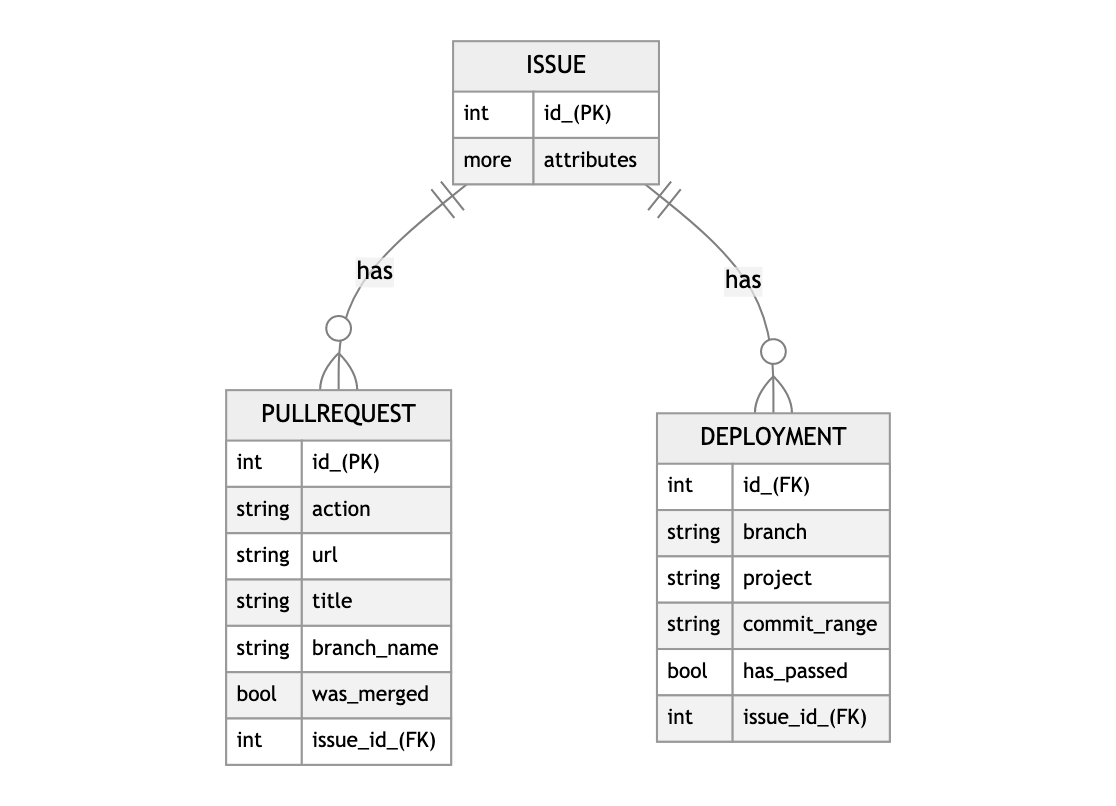
\includegraphics[width=0.8\textwidth]{images/erd/multiple.png}
    \label{fig:erd_multiple}
  \end{center}
\end{minipage}

\begin{minipage}{\textwidth}
  \subsubsection{Option 2: Inheritance}
  Die zweite Option ist, dass für Deployments und Pull-Requests keine eigenen Entitäten erstellt werden, sondern diese von
  einer gemeinsamen Entität erben. Das würde wie folgt aussehen:
  \begin{center}
    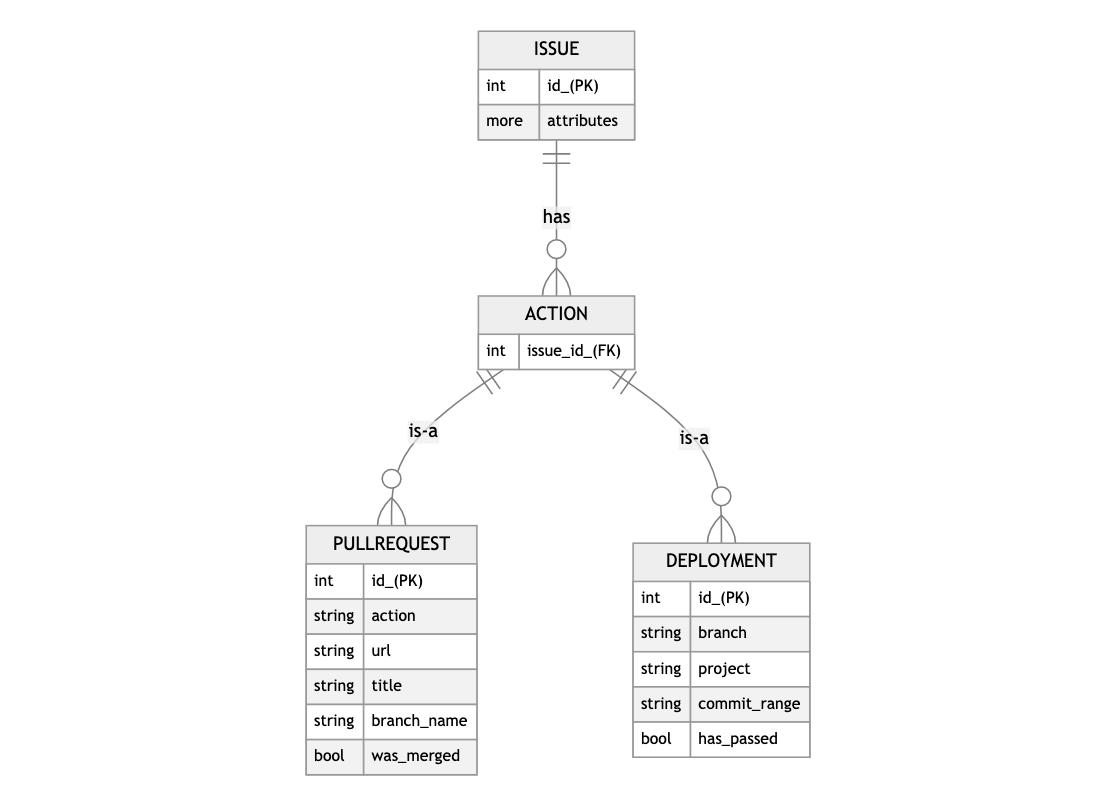
\includegraphics[width=0.8\textwidth]{images/erd/inheritance.png}
    \label{fig:erd_inheritance}
  \end{center}
\end{minipage}

\begin{minipage}{\textwidth}
  \subsection{Activity-Diagram}
  Das Activity-Diagramm zeigt den Ablauf des Plugins. In diesem Fall gibt es zwei Abläufe:
  \begin{itemize}
    \item Hook von SemaphoreCI oder GitHub
    \item Abfragen der Issues \newline
  \end{itemize}
\end{minipage}

\begin{minipage}{\textwidth}
  \subsubsection{Hook call}
  Die Hook calls werden von SemaphoreCI oder GitHub ausgelöst. Beide bei unterschiedlichen Events, welche beide mit Sanduhren
  dargestellt wurden:
  \begin{center}
    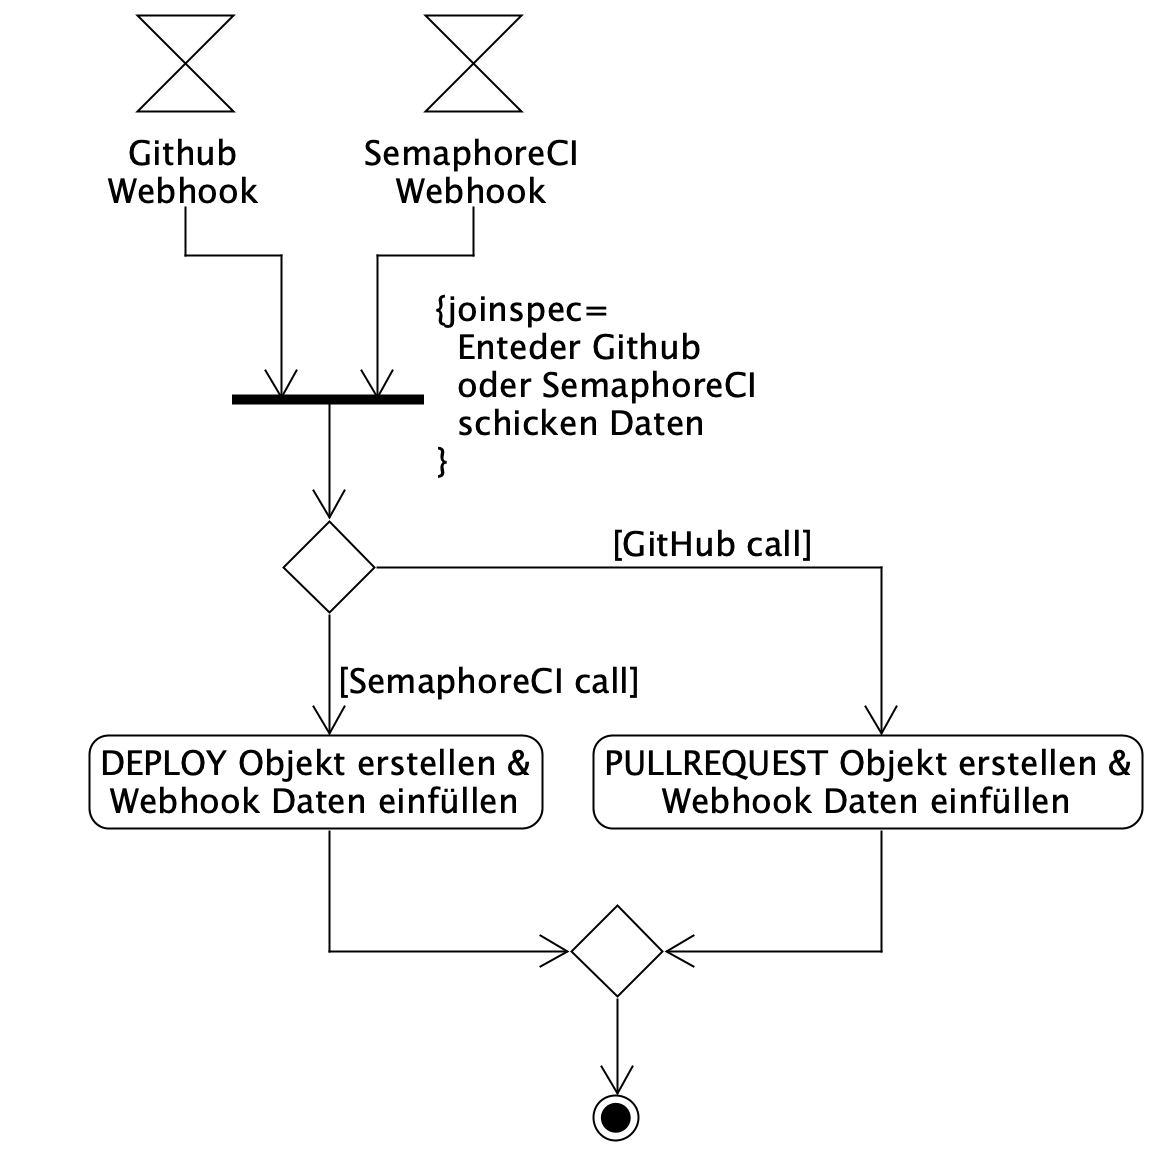
\includegraphics[width=0.8\textwidth]{images/activity/webhook.png}
    \label{fig:activity_hook_call}
  \end{center}
\end{minipage}

\begin{minipage}{\textwidth}
  \subsubsection{Abfrage der Issues}
  Falls der Nutzer auf die Details eines Issues klickt, wird eine Abfrage an das Plugin gesendet, welches die Pull Requests sowie
  Deployments abfragt und diese zurückgibt: \newline
  \begin{center}
    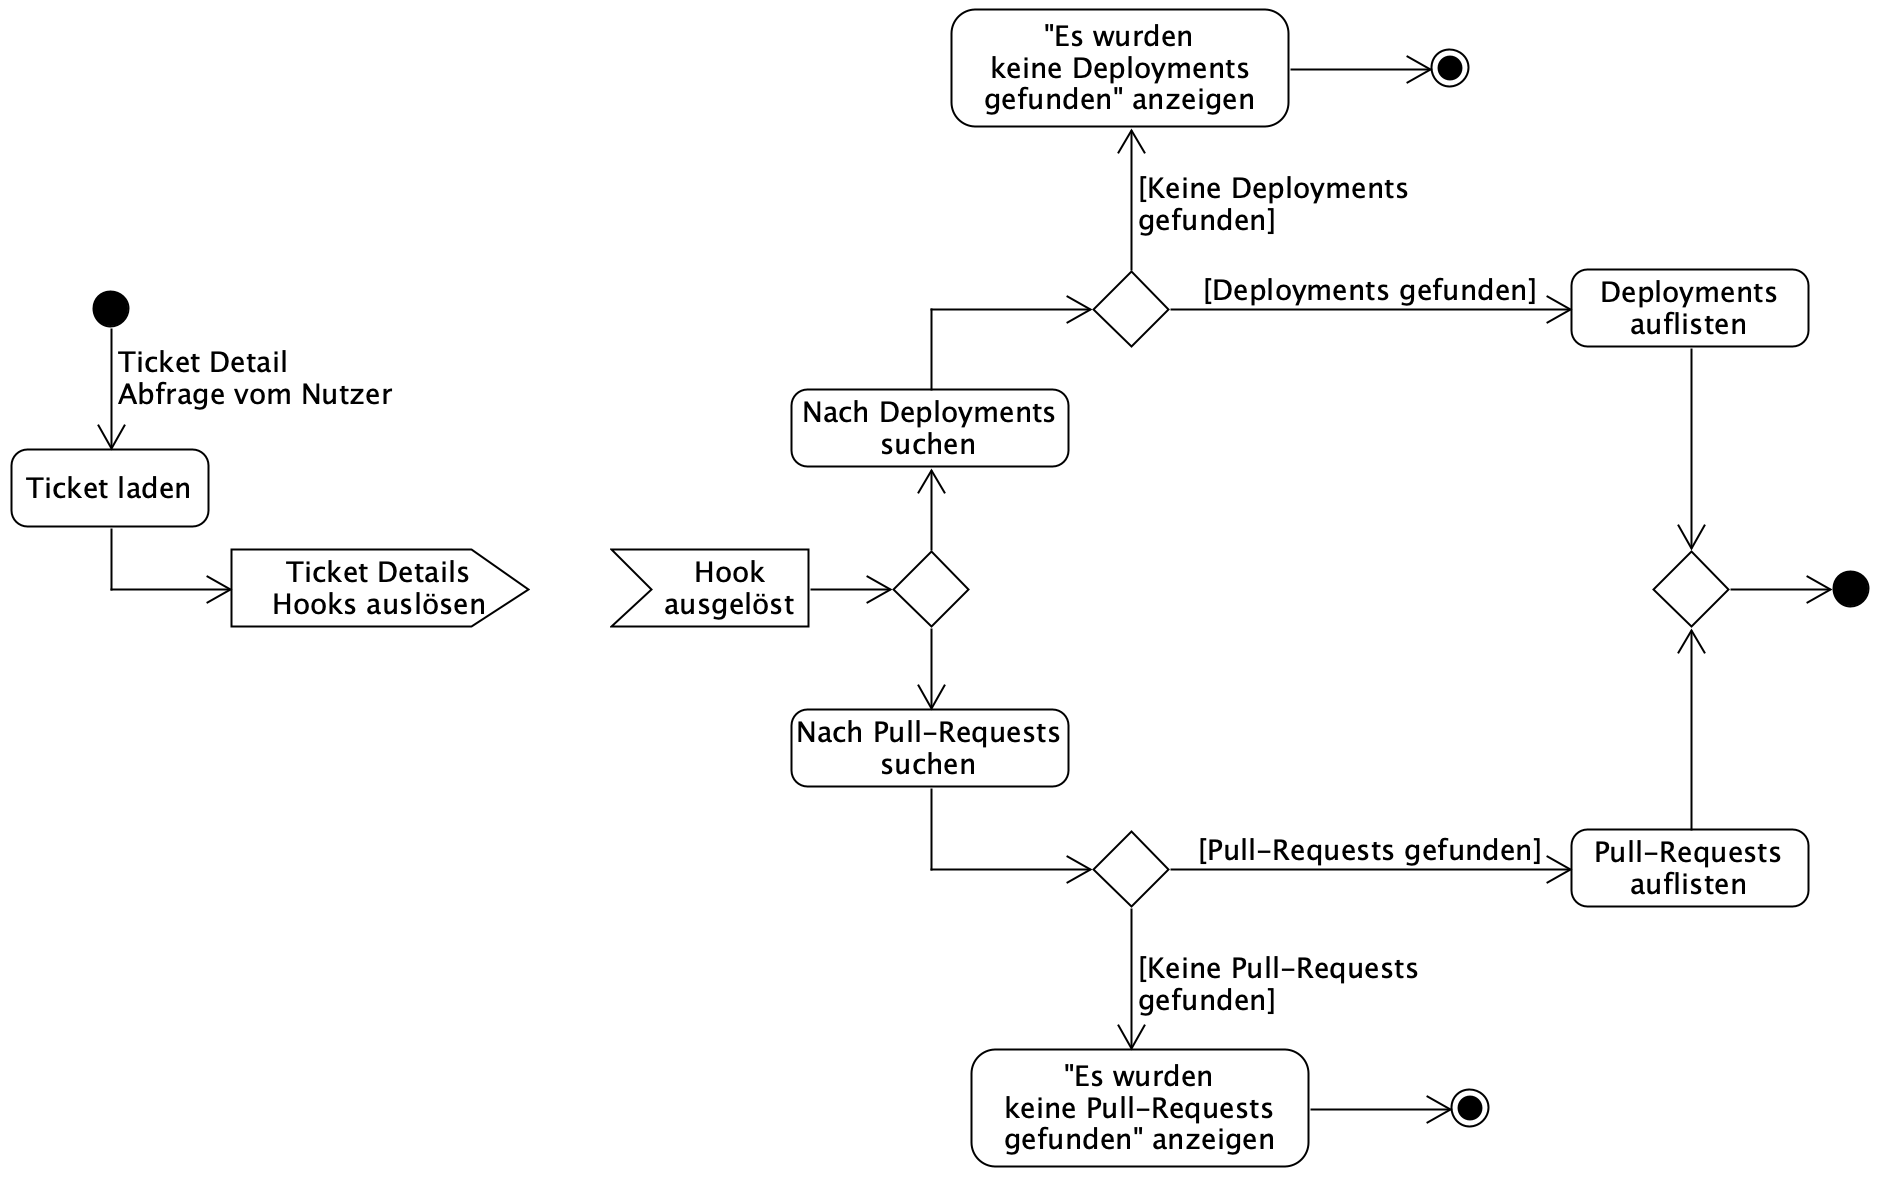
\includegraphics[width=0.8\textwidth]{images/activity/issues-view.png}
    \label{fig:activity_issues}
  \end{center}
\end{minipage}

\begin{minipage}{\textwidth}
  \subsection{Mockups}
  Damit die UI besser geplant werden kann, wird diese mit Mockups visualisiert. Diese Mockups sollen
  nur ungefähr wiedergeben, wie die UI aussehen soll. Da das Plugin auf einer bereits existierenden 
  Ansicht aufbaut, nämlich der Issue-View, wird diese nur sehr abstrahiert dargestellt. \newline
  Die bereits existierende Ansicht ist in der Abbildung mit weniger Opazität dargestellt. \newline
  \begin{center}
    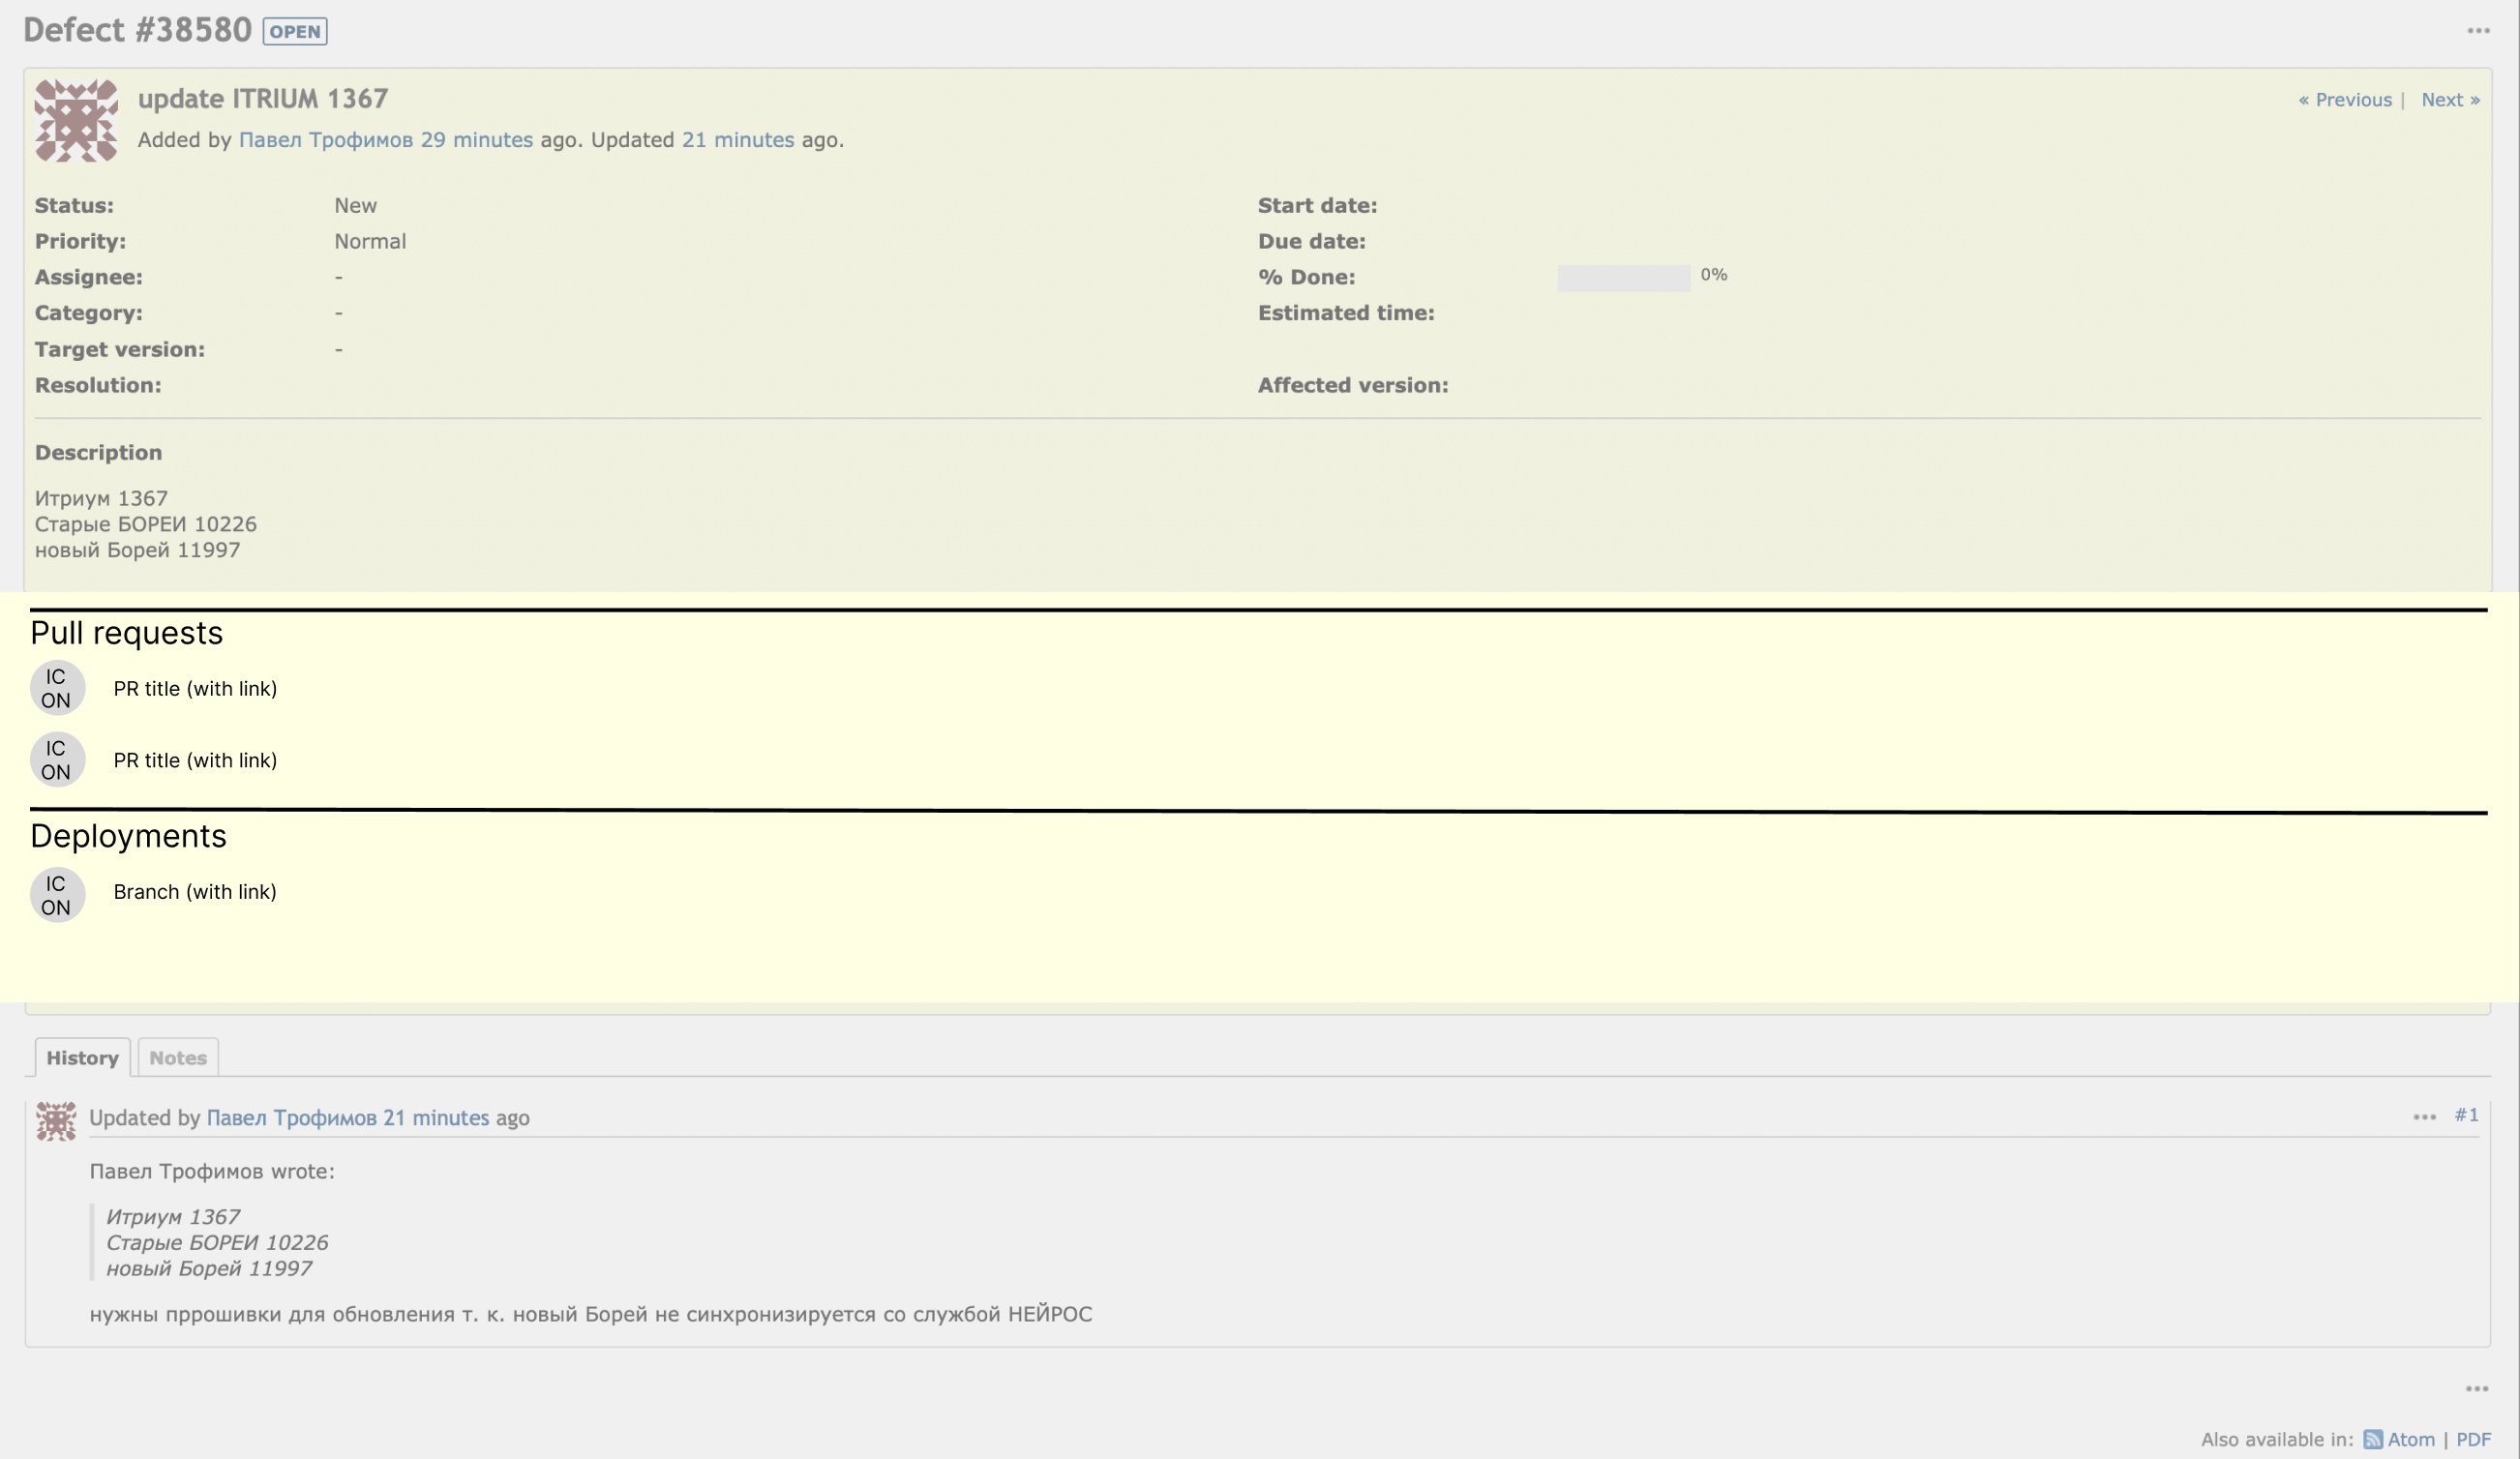
\includegraphics[width=0.8\textwidth]{images/mockup/details.png}
    \label{fig:mockup_details}
  \end{center}
\end{minipage}

\section{Testkonzept}
Das Testkonzept beschreibt, wie und mit welchen Werkzeugen das Resultat auf seine Richtigkeit kontrolliert wird.

\subsection{Testmethoden}
\subsubsection{Manuelle Tests}
\subsubsection{Automatisierte Tests}

\subsection{Testmittel}
